% !TEX root = ../main.tex
% File: chapters_part1/chap7_1.tex
% Nội dung cho Chương 7, Phần 1


\section{Các Metric kinh điển}
\label{sec:classic_metrics}

Đây là những công cụ đầu tiên và cơ bản nhất trong bộ công cụ của bất kỳ nhà thực hành NLP nào. Mỗi metric được thiết kế để đo lường một khía cạnh cụ thể của hiệu năng mô hình.

\subsection{Perplexity: Đo lường chất lượng của Mô hình Ngôn ngữ}
\label{ssec:perplexity}
\begin{itemize}
    \item \textbf{Dùng cho tác vụ nào?} Đánh giá chất lượng nội tại của các \textbf{Mô hình Ngôn ngữ (Language Models)} (ví dụ: các mô hình được huấn luyện để dự đoán từ tiếp theo).
    \item \textbf{Trực giác cốt lõi:} Một mô hình ngôn ngữ tốt là mô hình \textbf{ít "ngạc nhiên" (less surprised)} hơn khi nhìn thấy một câu văn thực tế. Perplexity (PPL), hay còn gọi là Độ bối rối, chính là một cách để định lượng sự "ngạc nhiên" này. \textbf{Perplexity càng thấp, mô hình càng tốt}.
    \item \textbf{Cơ chế hoạt động:} Perplexity có mối quan hệ trực tiếp với hàm mất mát Cross-Entropy. Đối với một chuỗi văn bản $W = (w_1, w_2, \dots, w_N)$, Perplexity được định nghĩa là:
        \begin{equation}
            \text{PPL}(W) = \sqrt[N]{\frac{1}{P(w_1, w_2, \dots, w_N)}} = \left( \prod_{i=1}^{N} \frac{1}{P(w_i|w_1, \dots, w_{i-1})} \right)^{1/N}
            \label{eq:perplexity}
        \end{equation}
        Về mặt toán học, nó là nghịch đảo của xác suất trung bình trên mỗi từ (được lấy căn bậc $N$).
    \item \textbf{Hạn chế:}
        \begin{itemize}
            \item Chỉ đo lường khả năng dự đoán xác suất, không trực tiếp đo lường chất lượng ngữ nghĩa hay sự mạch lạc của văn bản được sinh ra.
            \item Rất nhạy cảm với kích thước từ vựng. Không thể so sánh Perplexity của hai mô hình có từ vựng khác nhau.
        \end{itemize}
\end{itemize}

\subsection{Precision, Recall, và F1-Score: Nền tảng của các bài toán Phân loại}
\label{ssec:f1_score}
Đây là bộ ba metric không thể thiếu cho hầu hết các bài toán \textbf{phân loại (classification)} và \textbf{trích xuất thông tin (information extraction)} như NER.

\subsubsection{Các thành phần cơ bản}
Để hiểu bộ ba này, chúng ta cần định nghĩa bốn kết quả có thể xảy ra khi phân loại một điểm dữ liệu:
\begin{itemize}
    \item \textbf{True Positive (TP):} Dự đoán là \textbf{Dương tính}, và thực tế là \textbf{Dương tính}. (Dự đoán đúng)
    \item \textbf{True Negative (TN):} Dự đoán là \textbf{Âm tính}, và thực tế là \textbf{Âm tính}. (Dự đoán đúng)
    \item \textbf{False Positive (FP):} Dự đoán là \textbf{Dương tính}, nhưng thực tế là \textbf{Âm tính}. (Lỗi Loại I - "báo động giả")
    \item \textbf{False Negative (FN):} Dự đoán là \textbf{Âm tính}, nhưng thực tế là \textbf{Dương tính}. (Lỗi Loại II - "bỏ sót")
\end{itemize}

\begin{center}
    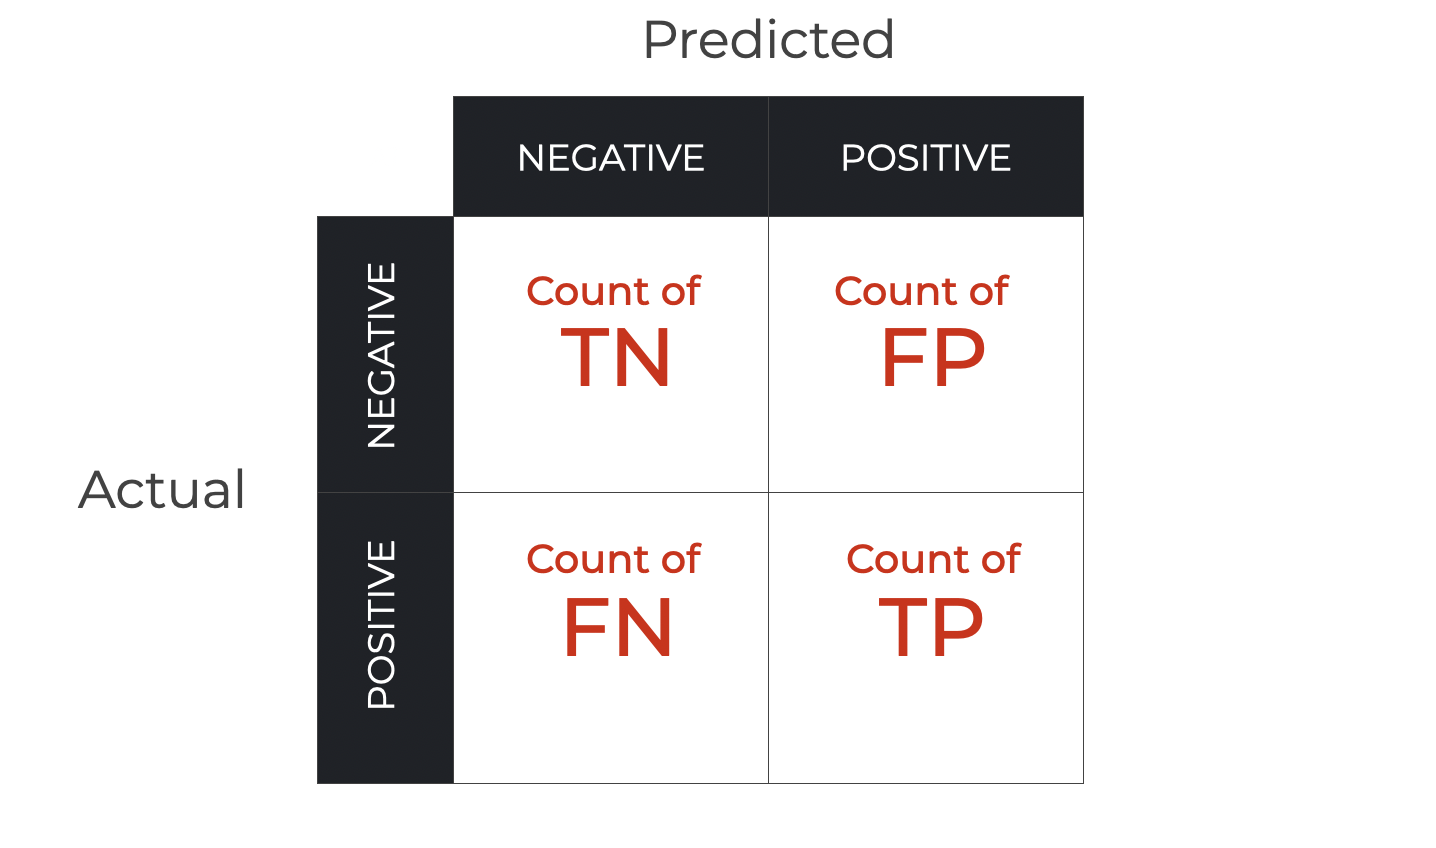
\includegraphics[width=0.6\textwidth]{confusion_matrix.png}
    \captionof{figure}{Ma trận nhầm lẫn (Confusion Matrix) minh họa bốn kết quả của một bài toán phân loại nhị phân.}
    \label{fig:confusion_matrix}
\end{center}

\subsubsection{Định nghĩa các Metric}
\paragraph{Precision (Độ chính xác)}
\begin{itemize}
    \item \textbf{Câu hỏi nó trả lời:} "Trong số tất cả những gì mô hình dự đoán là Dương tính, có bao nhiêu cái thực sự là Dương tính?"
    \item \textbf{Công thức:}
        $$ \text{Precision} = \frac{\text{TP}}{\text{TP} + \text{FP}} $$
    \item \textbf{Mục tiêu:} Tối đa hóa Precision có nghĩa là cố gắng giảm thiểu số lượng báo động giả (FP). Rất quan trọng trong các ứng dụng như phát hiện spam (thà bỏ sót một email spam còn hơn là đưa một email quan trọng vào hòm thư rác).
\end{itemize}

\paragraph{Recall (Độ phủ, hay Độ nhạy)}
\begin{itemize}
    \item \textbf{Câu hỏi nó trả lời:} "Trong số tất cả những cái thực sự là Dương tính, mô hình đã tìm thấy được bao nhiêu cái?"
    \item \textbf{Công thức:}
        $$ \text{Recall} = \frac{\text{TP}}{\text{TP} + \text{FN}} $$
    \item \textbf{Mục tiêu:} Tối đa hóa Recall có nghĩa là cố gắng giảm thiểu số lượng bỏ sót (FN). Rất quan trọng trong các ứng dụng như chẩn đoán y tế (thà chẩn đoán nhầm một người khỏe mạnh là có bệnh còn hơn là bỏ sót một người thực sự có bệnh).
\end{itemize}

\paragraph{F1-Score (Điểm F1)}
\begin{itemize}
    \item \textbf{Vấn đề:} Precision và Recall thường có sự đánh đổi (trade-off). Một mô hình rất "cẩn trọng" có thể có Precision cao nhưng Recall thấp, và ngược lại. F1-score được tạo ra để kết hợp cả hai thành một chỉ số duy nhất.
    \item \textbf{Công thức:} F1-score là trung bình điều hòa (harmonic mean) của Precision và Recall.
        $$ \text{F1-Score} = 2 \cdot \frac{\text{Precision} \cdot \text{Recall}}{\text{Precision} + \text{Recall}} $$
    \item \textbf{Mục tiêu:} F1-score cao khi cả Precision và Recall đều cao. Nó là một thước đo cân bằng, được sử dụng rộng rãi trong các tác vụ như NER, nơi chúng ta quan tâm đến cả việc không nhận dạng sai và không bỏ sót thực thể.
\end{itemize}
Khi đánh giá trên nhiều lớp, người ta thường tính `macro-F1` (tính F1 cho mỗi lớp rồi lấy trung bình) hoặc `micro-F1` (tính tổng TP, FP, FN trên tất cả các lớp rồi mới tính F1).

\subsection{BLEU: Đánh giá Dịch máy}
\label{ssec:bleu}
\begin{itemize}
    \item \textbf{Dùng cho tác vụ nào?} Chủ yếu là \textbf{Dịch máy (Machine Translation)}, nhưng đôi khi cũng dùng cho các tác vụ sinh văn bản khác.
    \item \textbf{Trực giác cốt lõi:} Một bản dịch tốt nên có nhiều \textbf{N-gram trùng lặp} với các bản dịch tham khảo chất lượng cao do con người tạo ra.
    \item \textbf{Cơ chế hoạt động:} BLEU (Bilingual Evaluation Understudy) tính toán một điểm số dựa trên hai yếu tố:
        \begin{enumerate}
            \item \textbf{Độ chính xác N-gram đã được sửa đổi (Modified N-gram Precision):} Tính toán tỷ lệ các N-gram (thường từ 1-gram đến 4-gram) trong câu do máy dịch tạo ra cũng xuất hiện trong các câu tham khảo. Nó được "sửa đổi" để ngăn mô hình lặp lại một từ đúng nhiều lần để gian lận điểm.
            \item \textbf{Hình phạt cho câu ngắn (Brevity Penalty - BP):} Nếu câu do máy dịch tạo ra ngắn hơn đáng kể so với các câu tham khảo, nó sẽ bị phạt. Điều này ngăn mô hình chỉ sinh ra một vài từ rất chính xác để có Precision cao.
        \end{enumerate}
        $$ \text{BLEU} = \text{BP} \cdot \exp\left(\sum_{n=1}^{N} w_n \log p_n\right) $$
        Trong đó $p_n$ là độ chính xác của n-gram, và $w_n$ thường là $1/N$.
    \item \textbf{Hạn chế:}
        \begin{itemize}
            \item \textbf{Chỉ quan tâm đến Precision, không quan tâm đến Recall:} Nó không phạt nếu bản dịch bỏ sót các thông tin quan trọng.
            \item \textbf{Không hiểu ngữ nghĩa:} Một bản dịch có thể dùng từ đồng nghĩa hoàn hảo nhưng vẫn bị điểm BLEU thấp nếu không khớp chính xác N-gram.
            \item \textbf{Gặp khó khăn với trật tự từ và sự sáng tạo:} Không đánh giá tốt các bản dịch có cấu trúc câu khác biệt nhưng vẫn đúng.
        \end{itemize}
\end{itemize}

\subsection{ROUGE: Đánh giá Tóm tắt Văn bản}
\label{ssec:rouge}
\begin{itemize}
    \item \textbf{Dùng cho tác vụ nào?} Chủ yếu là \textbf{Tóm tắt văn bản (Summarization)}.
    \item \textbf{Trực giác cốt lõi:} ROUGE (Recall-Oriented Understudy for Gisting Evaluation) hoạt động ngược lại với BLEU. Nó cho rằng một bản tóm tắt tốt nên \textbf "bao phủ" được các N-gram quan trọng có trong các bản tóm tắt tham khảo của con người.
    \item \textbf{Cơ chế hoạt động:} ROUGE là một họ các metric, trong đó phổ biến nhất là:
        \begin{itemize}
            \item \textbf{ROUGE-N:} Dựa trên sự trùng lặp N-gram, nhưng tính toán dựa trên \textbf{Recall}.
                $$ \text{ROUGE-N} = \frac{\text{Số N-gram trong tham khảo cũng xuất hiện trong tóm tắt máy}}{\text{Tổng số N-gram trong tham khảo}} $$
                Thường dùng `ROUGE-1` (unigram) và `ROUGE-2` (bigram).
            \item \textbf{ROUGE-L:} Dựa trên \textbf{Chuỗi con chung dài nhất (Longest Common Subsequence - LCS)}. Nó không yêu cầu các từ phải liền kề nhau, do đó nắm bắt được sự tương đồng về trật tự từ tốt hơn.
        \end{itemize}
    \item \textbf{Hạn chế:} Tương tự như BLEU, ROUGE cũng chỉ dựa trên sự khớp bề mặt của từ và không hiểu được ngữ nghĩa sâu sắc. Một bản tóm tắt có thể diễn đạt lại ý tưởng một cách hoàn hảo nhưng vẫn bị điểm ROUGE thấp.
\end{itemize}

Mặc dù có nhiều hạn chế, các metric kinh điển này vẫn được sử dụng rộng rãi vì chúng tự động, nhanh chóng và cung cấp một thước đo khách quan (dù không hoàn hảo) để so sánh các mô hình với nhau trong quá trình phát triển.